\documentclass[letterpaper,11pt]{article}

\usepackage[spanish,es-tabla]{babel}
\usepackage[utf8]{inputenc}
\usepackage[T1]{fontenc}
\usepackage{lmodern}
\usepackage[top=1.8cm,bottom=2.2cm,left=2.5cm,right=2.5cm,headheight=28pt,includehead,headsep=0.7cm]{geometry}
\usepackage{graphicx}
\usepackage{xcolor}
\usepackage{booktabs}
\usepackage{array}
\usepackage{float}
\usepackage{enumitem}
\usepackage{fancyhdr}
\usepackage{hyperref}
\usepackage{listings}
\usepackage{amsmath}
\usepackage{amssymb}
\usepackage{tikz}
\usepackage{caption}

\definecolor{verde}{RGB}{0,128,0}
\definecolor{azulmarino}{RGB}{0,0,128}
\definecolor{gris}{RGB}{95,95,95}
\definecolor{grisclaro}{RGB}{245,245,245}
\definecolor{codegreen}{rgb}{0,0.45,0}
\definecolor{codegray}{rgb}{0.45,0.45,0.45}
\definecolor{codepurple}{rgb}{0.45,0,0.65}
\definecolor{backcolor}{rgb}{0.96,0.96,0.94}

\hypersetup{
    colorlinks=true,
    linkcolor=azulmarino,
    urlcolor=azulmarino
}

\lstdefinestyle{mystyle}{
    backgroundcolor=\color{backcolor},
    commentstyle=\color{codegreen},
    keywordstyle=\color{magenta},
    numberstyle=\tiny\color{codegray},
    stringstyle=\color{codepurple},
    basicstyle=\ttfamily\footnotesize,
    breaklines=true,
    numbers=left,
    tabsize=4,
    showstringspaces=false
}
\lstset{style=mystyle}

\newcommand{\universidad}{Universidad Técnica Metropolitana}
\newcommand{\carrera}{Ingeniería Civil en Ciencia de Datos}
\newcommand{\codcurso}{INFB8090}
\newcommand{\nombrecurso}{Computación Paralela y Distribuida}
\newcommand{\fecha}{Mayo de 2026}
\newcommand{\profesor}{Michael Gabriel Miranda Sandoval}
\newcommand{\autor}{Welinton Barrera Mondaca \\ Joaquin Araya \\ Juan Toledo}
\newcommand{\encactividad}{Prueba 1 - Parte II grupal}
\newcommand{\descactividad}{Fundamentos de Computación Paralela, Concurrencia, Diseño Algorítmico y OpenMP}

\fancyhf{}
\fancyheadoffset[L]{0.4cm}
\fancyhead[L]{
\begin{tikzpicture}[remember picture,overlay]
    \fill[verde] (current page.north west) rectangle ++(\paperwidth/3,-0.18cm);
    \fill[azulmarino] ([xshift=\paperwidth/3]current page.north west) rectangle ++(\paperwidth*2/3,-0.18cm);
    \fill[azulmarino] (current page.south west) rectangle ++(\paperwidth*0.75,0.18cm);
    \fill[verde] ([xshift=0.75\paperwidth]current page.south west) rectangle ++(\paperwidth*0.25,0.18cm);
\end{tikzpicture}
\rmfamily \fontsize{9}{11}\selectfont
{\textcolor{verde}{\codcurso} -
\textcolor{azulmarino}{\nombrecurso}\\
\textcolor{gris}{\carrera}}
}
\fancyfoot[C]{
    \fontsize{7pt}{7pt}\selectfont \color{gris}
    \universidad\ - Parte II grupal \hfill \thepage
}
\renewcommand{\headrulewidth}{0pt}
\renewcommand{\footrulewidth}{0.05pt}

\begin{document}
\pagestyle{fancy}

\begin{titlepage}
    \centering
    \vspace*{1.4cm}
    
\includegraphics[width=3.1cm]{logos_utem/utem.jpg}
    \vspace{1.2cm}

    {\Large \textcolor{verde}{\codcurso} - \textcolor{azulmarino}{\nombrecurso}\par}
    \vspace{0.2cm}
    {\large \textcolor{gris}{\carrera}\par}
    \vspace{2.2cm}

    {\LARGE\bfseries \encactividad\par}
    \vspace{0.5cm}
    {\large\itshape ``\descactividad''\par}
    \vspace{2.0cm}

    \begin{tabular}{rl}
        Integrantes: & Welinton Barrera Mondaca \\
                     & Joaquin Araya \\
                     & Juan Toledo \\
        Profesor: & \profesor \\
        Sección: & 412 \\
        Fecha: & \fecha \\
    \end{tabular}

    \vfill
    {\universidad\par}
\end{titlepage}

\tableofcontents
\newpage

\section*{Resumen ejecutivo}
\addcontentsline{toc}{section}{Resumen ejecutivo}

Para la parte grupal trabajamos los tres ejercicios pedidos por la prueba desde una misma idea: no elegir la herramienta antes de mirar la forma del problema. En normalización masiva usamos OpenMP porque el cálculo recorre una matriz grande en memoria compartida y necesita reducciones por columna. En logs comprimidos elegimos un pipeline híbrido, con agregación parcial por lotes, porque la lectura y descompresión se mezclan con parseo JSON, limpieza y reducción por ventanas. Para embeddings usamos bloques y top-\(k\) incremental, evitando construir una matriz completa de similitud.

Los datos se generaron de forma sintética y reproducible, tomando como referencia fuentes públicas poco genéricas: variables de tráfico aéreo tipo OpenSky para la normalización, estructura de autenticación/logs de RBA y Azure Application Gateway para el pipeline, y el formato SIFT1M para embeddings de dimensión 128. Esta decisión no contradice el enunciado, porque la pauta permite dataset público o generación sintética. La ventaja práctica es que los tamaños pedidos se pueden reproducir con semilla fija sin depender de descargas grandes o inestables.

Las mediciones se realizaron en Windows 11, CPU AMD Ryzen 7 6800H, 8 núcleos físicos, 16 hilos lógicos y 15,26 GiB de RAM. Los benchmarks principales quedaron en anexos CSV. Para OpenMP se midió la matriz completa solicitada, \(50.000.000 \times 16\), con 1, 2, 4 y 8 hilos. Para logs se midió una muestra comprimida de 16 MiB, dejando el generador parametrizado para 2 GiB. Para embeddings sí se ejecutó el tamaño completo solicitado de \(20.000 \times 128\).

\section*{Punto de partida individual del grupo}
\addcontentsline{toc}{section}{Punto de partida individual del grupo}

Para contrastar la parte grupal con la primera mitad de la prueba, revisamos las fotografías disponibles de la respuesta individual de Welinton. Joaquin y Juan no tuvieron oportunidad de sacar fotografías a sus pruebas, por lo que esa evidencia no quedó registrada. Dejamos esta limitación explícita para que la comparación no parezca simétrica donde no lo es; aun así, la discusión grupal posterior permitió revisar las decisiones técnicas de los tres integrantes antes de cerrar las soluciones.

En las respuestas de Welinton aparece una línea de trabajo que se mantuvo en el informe grupal: antes de paralelizar hay que diagnosticar el cuello de botella y no asumir que más hilos siempre reduce el tiempo. En OpenMP se reconoce el riesgo de carreras al actualizar acumuladores compartidos, como conteos o sumas por columna, lo que calza con la decisión final de usar arreglos privados por hilo y una combinación controlada al final. En Python, la respuesta individual separa lectura/descompresión, parseo/limpieza y agregación, criterio que después se transformó en el benchmark de estrategias secuencial, por hilos, por procesos e híbrida. Para el ejercicio de embeddings, el apunte individual deja ver la preocupación por bloquear el cálculo y no guardar una matriz completa de similitudes, que es la misma restricción que guió el top-\(k\) incremental por bloques.

\section{Ejercicio 1: normalización masiva con OpenMP}

\subsection{Diagnóstico del problema}

El ejercicio pide normalizar una matriz \(X\) de \(50.000.000 \times 16\) con valores faltantes representados como \texttt{NaN}. El tamaño no es complicado por cantidad de columnas, sino por el volumen total: \(800.000.000\) valores. Si se usa \texttt{double}, la matriz ocupa cerca de 6,4 GB solo para los datos. Eso obliga a evitar copias innecesarias y a recorrer la memoria de manera secuencial por filas para mantener buena localidad.

La normalización por columna necesita dos fases naturales. Primero se calculan conteo, suma y suma de cuadrados ignorando \texttt{NaN}. Luego se transforma cada valor válido usando:

\[
z_{ij} = \frac{x_{ij} - \mu_j}{\sigma_j}
\]

La dependencia importante está en los acumuladores por columna. Si varios hilos actualizan una misma suma al mismo tiempo aparece una condición de carrera. Por eso el diseño no puede ser simplemente un \texttt{parallel for} con sumas compartidas.

\subsection{Datos usados}

Se implementó una matriz sintética reproducible con semilla 4128090. Las columnas simulan rangos numéricos similares a datos de seguimiento aéreo: latitud, longitud, velocidad, altitud, razón vertical, rumbo y otras señales continuas. La referencia conceptual es OpenSky, porque ofrece datos públicos de seguimiento aéreo y no corresponde a un dataset típico de clasificación usado por muchos grupos.

Los \texttt{NaN} se inyectan con una tasa de 3,5\%. En la verificación de escala completa se generaron \(772.004.542\) valores válidos de \(800.000.000\), consistente con esa tasa.

\subsection{Estrategias comparadas}

\begin{table}[H]
\centering
\caption{Comparación de estrategias para normalización}
\begin{tabular}{p{0.25\linewidth} p{0.34\linewidth} p{0.31\linewidth}}
\toprule
Estrategia & Ventaja & Límite principal \\
\midrule
Secuencial & Simple y determinista. Sirve como línea base. & No usa los núcleos disponibles y queda limitado por un solo hilo. \\
\texttt{parallel for} con \texttt{critical} & Evita la carrera de datos de forma directa. & Muy mala opción: cada elemento válido compite por entrar a la región crítica. \\
Acumuladores privados por hilo & Reduce la contención y permite combinar al final. & Usa arreglos auxiliares por hilo, aunque pequeños: \(hilos \times 16\). \\
Reducción por arreglo & Código más compacto si el compilador lo soporta bien. & Menos portable entre compiladores y versiones de OpenMP para arreglos dinámicos. \\
\bottomrule
\end{tabular}
\end{table}

Seleccionamos acumuladores privados por hilo porque dejan explícito qué es privado y qué se combina. Cada hilo recorre filas, acumula en sus 16 posiciones locales, y recién al terminar se fusionan los parciales. La transformación posterior no necesita sincronización porque cada celda se escribe una sola vez.

\subsection{Fragmento de implementación}

Para la configuración de C/C++ tomamos como referencia el material portable entregado por el profesor en \texttt{OpenMP.rar}: el instructivo de uso con \texttt{w64devkit}, la estructura de trabajo para VSCode y los ejemplos base \texttt{suma\_50M.c} y \texttt{primos\_pesado.c}. No copiamos esos programas como solución final; los usamos para mantener la misma forma de compilar, medir tiempo con OpenMP y separar correctamente la parte serial, paralela y de reducción.

El archivo desarrollado es \texttt{codigo\_openmp/normalizacion.cpp}. El comando usado fue:

\begin{lstlisting}[language=bash]
g++ -O3 -std=c++20 -fopenmp normalizacion.cpp -o normalizacion.exe
\end{lstlisting}

La idea central del cálculo de estadísticos es esta:

\begin{lstlisting}[language=C++]
#pragma omp parallel
{
    int tid = omp_get_thread_num();
    double* local_sum = thread_sums.data() + tid * cols;
    double* local_sum_sq = thread_sums_sq.data() + tid * cols;
    uint64_t* local_count = thread_counts.data() + tid * cols;

    #pragma omp for schedule(static)
    for (int64_t r = 0; r < static_cast<int64_t>(rows); ++r) {
        size_t base = static_cast<size_t>(r) * cols;
        for (int c = 0; c < cols; ++c) {
            double value = x[base + c];
            if (!std::isnan(value)) {
                local_sum[c] += value;
                local_sum_sq[c] += value * value;
                local_count[c] += 1;
            }
        }
    }
}
\end{lstlisting}

No se usa \texttt{critical} dentro del ciclo principal. Si se protegiera cada suma con \texttt{critical}, el acceso a los acumuladores quedaría serializado y el costo de sincronización aparecería justo en la parte más repetida del programa. En este caso eso significaría cientos de millones de entradas a una región crítica.

\subsection{Benchmark y análisis}

Para comparar 1, 2, 4 y 8 hilos se usó la matriz completa del enunciado, \(50.000.000 \times 16\), con tres repeticiones por configuración. El tiempo reportado corresponde a la normalización propiamente tal: cálculo de estadísticos y transformación. No se mezcla con la generación sintética de la matriz ni con la validación posterior, porque esos pasos sirven para reproducir y revisar el experimento, pero no forman parte del algoritmo que se quiere comparar.

\begin{table}[H]
\centering
\caption{Benchmark OpenMP con matriz \(50.000.000 \times 16\)}
\begin{tabular}{rrrrrr}
\toprule
Hilos & Tiempo (s) & Fit (s) & Transform (s) & Speedup & Eficiencia \\
\midrule
1 & 3,091 & 1,318 & 1,772 & 1,00 & 1,00 \\
2 & 4,278 & 2,695 & 1,583 & 0,72 & 0,36 \\
4 & 3,124 & 2,122 & 1,002 & 0,99 & 0,25 \\
8 & 1,817 & 1,254 & 0,563 & 1,70 & 0,21 \\
\bottomrule
\end{tabular}
\end{table}

La Figura 1 muestra el mismo resultado en forma visual. El punto más relevante no es solo que 8 hilos sea más rápido, sino que la eficiencia baja con fuerza, señal de que el límite práctico está más cerca del ancho de banda de memoria y de la combinación de parciales que del cálculo aritmético.

\begin{figure}[H]
    \centering
    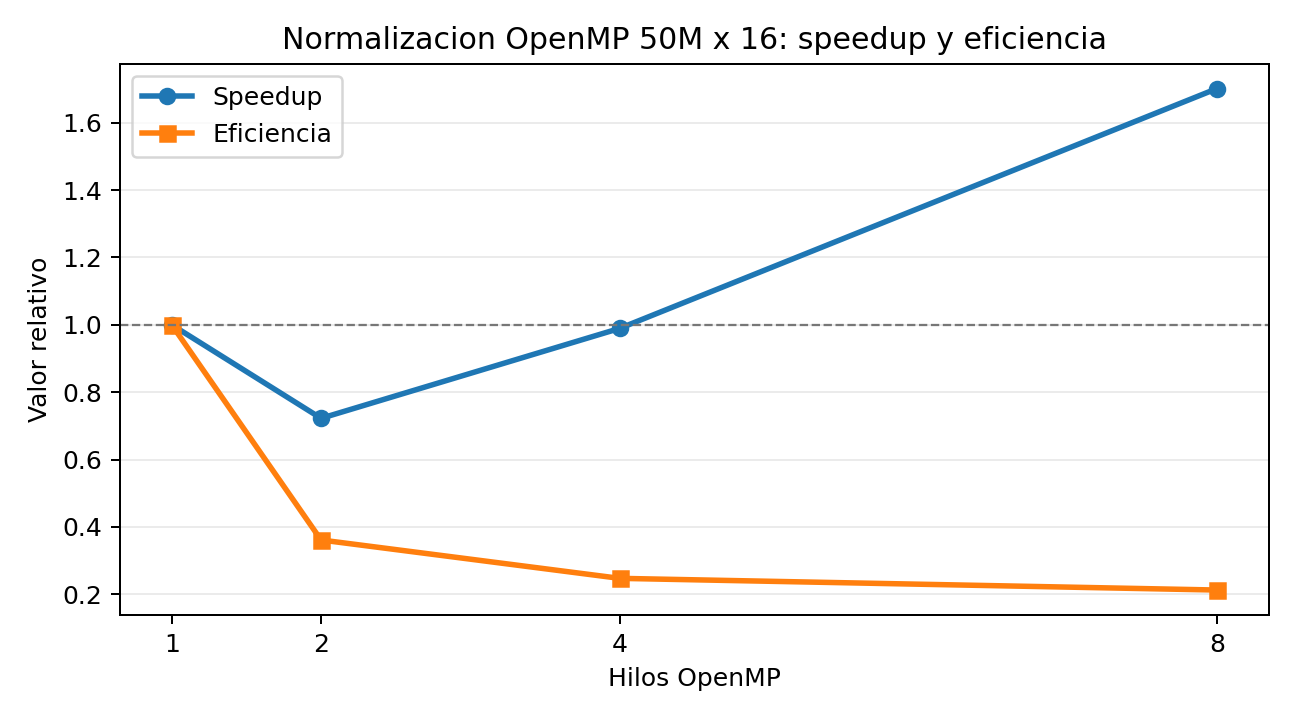
\includegraphics[width=0.82\linewidth]{figuras/openmp_speedup_eficiencia.png}
    \caption{Speedup y eficiencia de la normalización OpenMP.}
\end{figure}

El resultado no es lineal, y en el tamaño completo esa lectura se vuelve más visible. La transformación escala mejor que el cálculo de estadísticos, porque solo lee, normaliza y escribe cada celda. La fase de acumulación queda más expuesta al ancho de banda de memoria, a la localidad de caché y a la combinación de parciales. Por eso 2 y 4 hilos no mejoran la línea base en estas corridas, mientras que 8 hilos sí reducen el tiempo total. No lo interpretamos como una falla del diseño, sino como una señal de que el problema está cerca del límite de memoria del equipo usado.

La variación numérica se controló validando la matriz normalizada. En las corridas registradas, el máximo valor absoluto de media posterior y el máximo error de desviación estándar quedaron reportados como 0,000000 a seis decimales. Aun así, el orden de reducción en punto flotante puede cambiar los últimos bits, por lo que no conviene exigir igualdad binaria entre la versión secuencial y paralela.

\subsection{Riesgos y límites}

El cuello de botella más probable es memoria, no cómputo puro. Si se aumenta la cantidad de columnas, si se guardan copias de la matriz o si se usa \texttt{float64} junto con estructuras auxiliares grandes, el programa puede empezar a paginar. También cambiaría la decisión si las columnas fueran miles: en ese caso habría que revisar la forma de acumular, posiblemente por bloques de columnas o usando reducción vectorizada más específica.

\section{Ejercicio 2: pipeline concurrente de logs en Python}

\subsection{Diagnóstico del pipeline}

El pipeline pedido incluye lectura, descompresión, parseo, limpieza y agregación por ventanas temporales. No todas esas etapas tienen el mismo comportamiento. La lectura desde disco y parte de la descompresión son I/O-bound o se benefician de llamadas en C que pueden liberar el GIL. En cambio, el parseo JSON, la validación de campos y la actualización de diccionarios de agregación son trabajo CPU-bound dentro del intérprete.

Por ese motivo no sería correcto decir que \texttt{ThreadPoolExecutor} siempre sirve por tratarse de archivos. Si el cuello de botella real pasa a ser \texttt{json.loads} y manipulación de diccionarios, los hilos compiten bajo el GIL y la mejora puede desaparecer.

\subsection{Datos usados}

El generador produce archivos \texttt{.jsonl.gz} con:

\begin{itemize}[itemsep=0.1cm]
    \item \texttt{user\_id}
    \item \texttt{timestamp}
    \item \texttt{endpoint}
    \item \texttt{latency\_ms}
    \item \texttt{status\_code}
\end{itemize}

La forma de los datos se inspiró en dos fuentes públicas: RBA, por su estructura de eventos de autenticación con usuarios, y Azure Application Gateway, por el esquema de logs HTTP con duración, URI y código de respuesta. La muestra local usada para benchmark fue de 16 MiB comprimidos, con 1.300.000 eventos. El script \texttt{generar\_logs.py} queda parametrizado para producir 2 GiB comprimidos:

\begin{lstlisting}[language=bash]
python generar_logs.py --out-dir datos_logs_2gib --target-mb 2048 --files 32
\end{lstlisting}

\subsection{Comparación de estrategias}

\begin{table}[H]
\centering
\caption{Opciones evaluadas para el pipeline}
\begin{tabular}{p{0.23\linewidth} p{0.34\linewidth} p{0.33\linewidth}}
\toprule
Opción & Cuándo tendría sentido & Problema observado o esperado \\
\midrule
Secuencial & Línea base estable y fácil de auditar. & No solapa etapas ni usa varios núcleos. \\
\texttt{ThreadPoolExecutor} & Varios archivos, lectura lenta o descompresión dominante. & El parseo JSON y la agregación quedan limitados por el GIL. \\
\texttt{ProcessPoolExecutor} por archivo & Archivos independientes y parseo CPU-bound. & Duplica inicialización y serializa resultados parciales. \\
Híbrido por lotes & Lectura por streaming y parseo/agregación en procesos. & Si el lote es muy pequeño domina el costo de comunicación; si es muy grande sube la memoria. \\
\bottomrule
\end{tabular}
\end{table}

Se evaluó si convenía incluir \texttt{asyncio} como cuarta opción. Se descartó porque las etapas que dominan el tiempo en este pipeline son la descompresión \texttt{gzip} y el parseo JSON, ambas CPU-bound bajo GIL, que no liberan el intérprete el tiempo suficiente como para que el solapamiento cooperativo de \texttt{asyncio} mejore el tiempo total. En este escenario \texttt{asyncio} competiría con los hilos del kernel sin aportar paralelismo real de CPU; tendría sentido si el cuello de botella fuera espera de red o disco lento, no lo es para archivos locales pequeños y descompresión intensiva.

La estrategia seleccionada para el diseño final es híbrida por lotes: lectura/descompresión en streaming, partición en bloques de líneas y parseo/agregación en procesos. Cada worker devuelve agregados parciales por clave \((ventana, endpoint)\). El proceso principal combina esos parciales sumando conteos, latencias acumuladas, máximos y errores 5xx.

\begin{figure}[H]
    \centering
    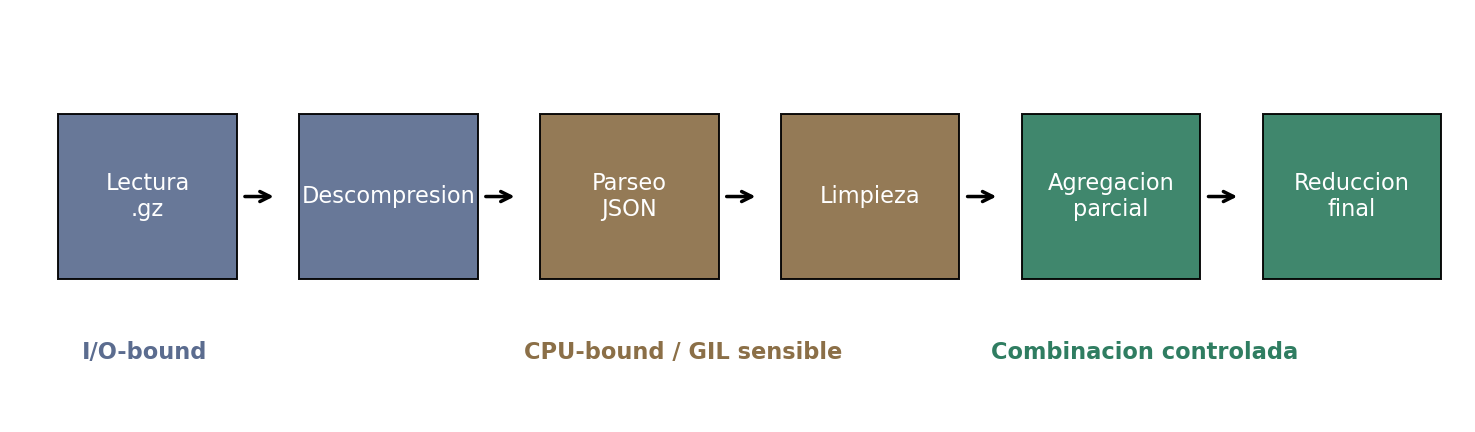
\includegraphics[width=0.95\linewidth]{figuras/pipeline_logs_diagrama.png}
    \caption{Diseño conceptual del pipeline concurrente de logs.}
\end{figure}

\subsection{Agregación parcial}

La agregación usa ventanas de 5 minutos. Para cada clave se mantiene:

\[
(\text{conteo},\ \text{suma latencia},\ \text{latencia máxima},\ \text{errores 5xx})
\]

No se comparten diccionarios entre procesos. Eso evita inconsistencias y bloqueos. La combinación final es determinista porque las operaciones son asociativas para conteos y sumas; en máximos se usa \(\max\). La suma de latencias puede tener pequeñas variaciones de punto flotante si se cambia el orden, pero no afecta las métricas agregadas al nivel de precisión usado.

\subsection{Benchmark}

El benchmark usó 2 repeticiones por configuración y una corrida de calentamiento. Se controló que todas las estrategias entregaran la misma firma: 1.300.000 requests, 56.404 grupos de agregación y mismo total de errores.

\begin{table}[H]
\centering
\caption{Benchmark de pipeline sobre logs comprimidos de 16 MiB}
\begin{tabular}{lrrrrr}
\toprule
Estrategia & Workers & Tiempo (s) & Speedup & Eficiencia & Req/s \\
\midrule
Secuencial & 1 & 10,129 & 1,00 & 1,00 & 128.342 \\
ThreadPool & 4 & 11,656 & 0,87 & 0,22 & 111.535 \\
ProcessPool & 4 & 3,744 & 2,71 & 0,68 & 347.230 \\
ProcessPool & 8 & 2,732 & 3,71 & 0,46 & 475.764 \\
Híbrido lotes & 4 & 3,740 & 2,71 & 0,68 & 347.602 \\
Híbrido lotes & 8 & 3,631 & 2,79 & 0,35 & 357.994 \\
\bottomrule
\end{tabular}
\end{table}

La Figura 3 deja más claro el patrón: los hilos no reducen el tiempo total en esta carga, mientras que los procesos bajan el tiempo cuando el parseo y la agregación pesan más que la lectura. El enfoque híbrido queda competitivo en 4 workers, pero con 8 workers paga más coordinación por lotes.

\begin{figure}[H]
    \centering
    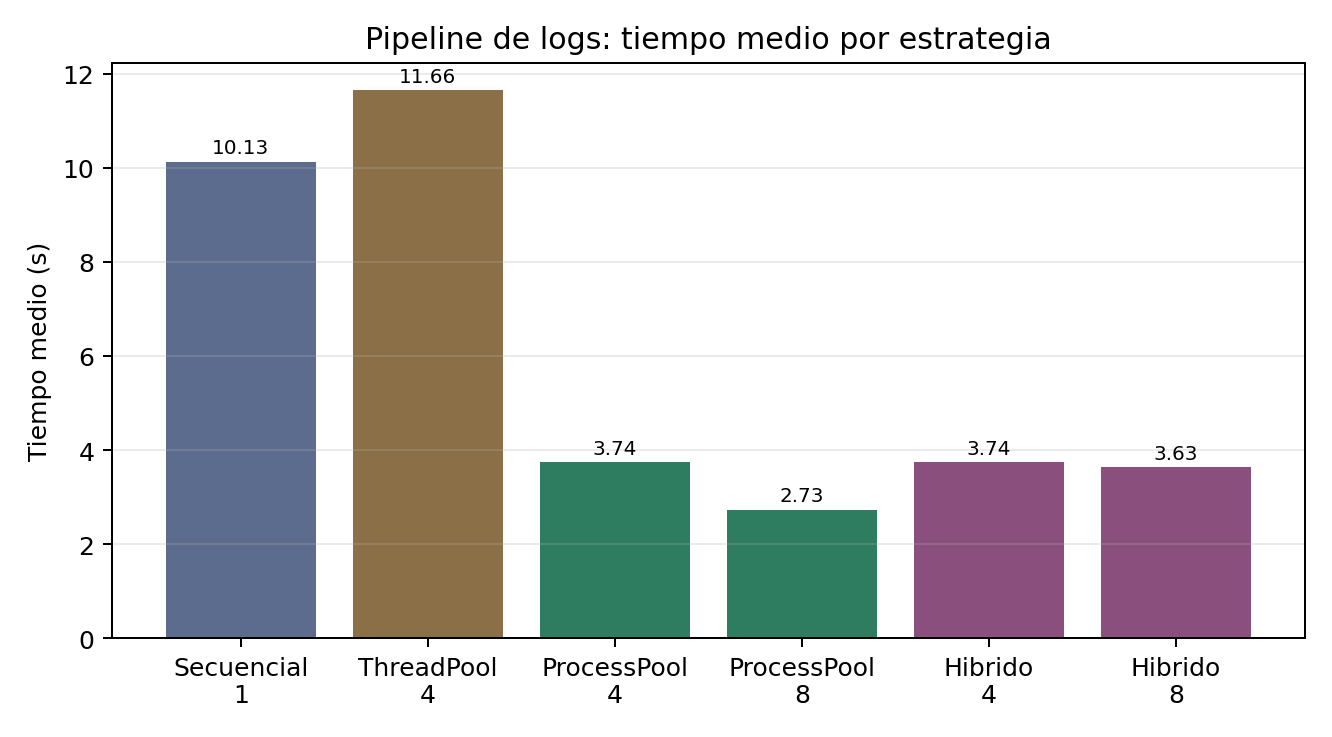
\includegraphics[width=0.86\linewidth]{figuras/logs_tiempo_estrategia.png}
    \caption{Tiempo medio por estrategia en el pipeline de logs.}
\end{figure}

Los hilos no mejoraron porque la carga local no estuvo dominada por espera de disco. El parseo JSON y la agregación en Python pesaron lo suficiente para que el GIL limitara el avance real. Los procesos sí mejoraron, sobre todo hasta 4 workers. Con 8 workers el \texttt{ProcessPool} siguió bajando tiempo, pero con eficiencia menor por serialización y coordinación. El híbrido por lotes fue competitivo con 4 workers, aunque con 8 perdió frente al proceso por archivo, principalmente porque enviar lotes de strings entre procesos agrega tráfico de copia.

\subsection{Riesgos y condiciones de cambio}

Si los archivos reales fueran pocos y enormes, convendría particionar por offsets o por bloques de líneas, no solo por archivo. Si la descompresión dominara, los hilos podrían recuperar valor. Si la agregación creciera demasiado, habría que reducir cardinalidad antes de devolver parciales o escribir resultados intermedios en disco. El tamaño de lote también es sensible: lotes pequeños aumentan overhead y lotes grandes suben memoria y latencia de combinación.

\section{Ejercicio 3: similitud por bloques para embeddings}

\subsection{Diagnóstico y memoria}

El ejercicio pide 20.000 vectores de dimensión 128 normalizados a norma 1. Si la similitud es coseno, al estar normalizados basta usar producto punto. La forma directa sería construir la matriz:

\[
S = E E^T
\]

con \(E \in \mathbb{R}^{20000 \times 128}\). La matriz completa tiene \(20.000^2 = 400.000.000\) similitudes. En \texttt{float32} ocupa cerca de 1,49 GiB; en \texttt{float64}, 2,98 GiB. Eso no incluye índices, top-\(k\), estructuras auxiliares ni memoria temporal de BLAS. En un equipo de 16 GiB podría caber una vez, pero no es una buena estrategia: escala cuadráticamente y deja poco margen.

\subsection{Datos usados}

Se generaron 20.000 vectores sintéticos de dimensión 128 con semilla fija y normalización a norma 1. El formato se eligió siguiendo SIFT1M, que es una referencia pública clásica para búsqueda de vecinos aproximados/exactos con vectores de 128 dimensiones. La generación agrega pequeños grupos latentes para que existan vecinos cercanos reales y el top-\(k\) no sea ruido uniforme.

\subsection{Estrategia seleccionada}

La estrategia final procesa bloques de filas contra bloques de columnas. Para cada bloque de filas se mantiene un top-10 local:

\begin{enumerate}[itemsep=0.1cm]
    \item Tomar un bloque \(B_i\) de filas.
    \item Calcular \(B_i \cdot B_j^T\) contra cada bloque de columnas.
    \item Anular la diagonal cuando se compara un vector consigo mismo.
    \item Fusionar candidatos del bloque con el top-10 acumulado.
    \item Guardar solo índices y puntajes top-10 por vector.
\end{enumerate}

Con bloque 1024, la matriz temporal tiene \(1024^2\) valores, cerca de 4 MiB en \texttt{float32}. Esa diferencia es la razón principal para no construir la matriz completa.

\subsection{Paralelización}

Se paralelizaron bloques de filas usando procesos y memoria compartida. Los embeddings se copian una vez a \texttt{multiprocessing.shared\_memory}; cada proceso lee la misma matriz y devuelve solo top-10 para su rango de filas. Esta decisión evita copiar \(20.000 \times 128\) valores a cada tarea. También evita compartir estructuras mutables de top-\(k\), porque cada proceso escribe resultados de filas distintas.

El balance de carga es simple porque cada fila compara contra todos los vectores, por lo que el costo por bloque es bastante uniforme. La localidad de memoria se cuida manteniendo bloques contiguos y usando multiplicación matricial de NumPy para que el trabajo interno quede en rutinas optimizadas.

\subsection{Benchmark y calidad}

La métrica de calidad fue exactitud del top-10 sobre una muestra de validación por fuerza bruta. Como la estrategia por bloques es exacta, la coincidencia fue 1,000000.

\begin{table}[H]
\centering
\caption{Benchmark top-10 exacto para \(20.000 \times 128\)}
\begin{tabular}{rrrrrr}
\toprule
Workers & Tiempo (s) & Speedup & Eficiencia & Comparaciones/s & Recall top-10 \\
\midrule
1 & 4,792 & 1,00 & 1,00 & 83.465.802 & 1,00 \\
2 & 2,998 & 1,60 & 0,80 & 133.396.255 & 1,00 \\
4 & 1,874 & 2,56 & 0,64 & 213.444.506 & 1,00 \\
\bottomrule
\end{tabular}
\end{table}

La Figura 4 resume la relación entre tiempo y speedup. El resultado es favorable para 4 workers, aunque no lineal, lo que calza con el costo de coordinar procesos y mover los top-\(k\) parciales de vuelta al proceso principal.

\begin{figure}[H]
    \centering
    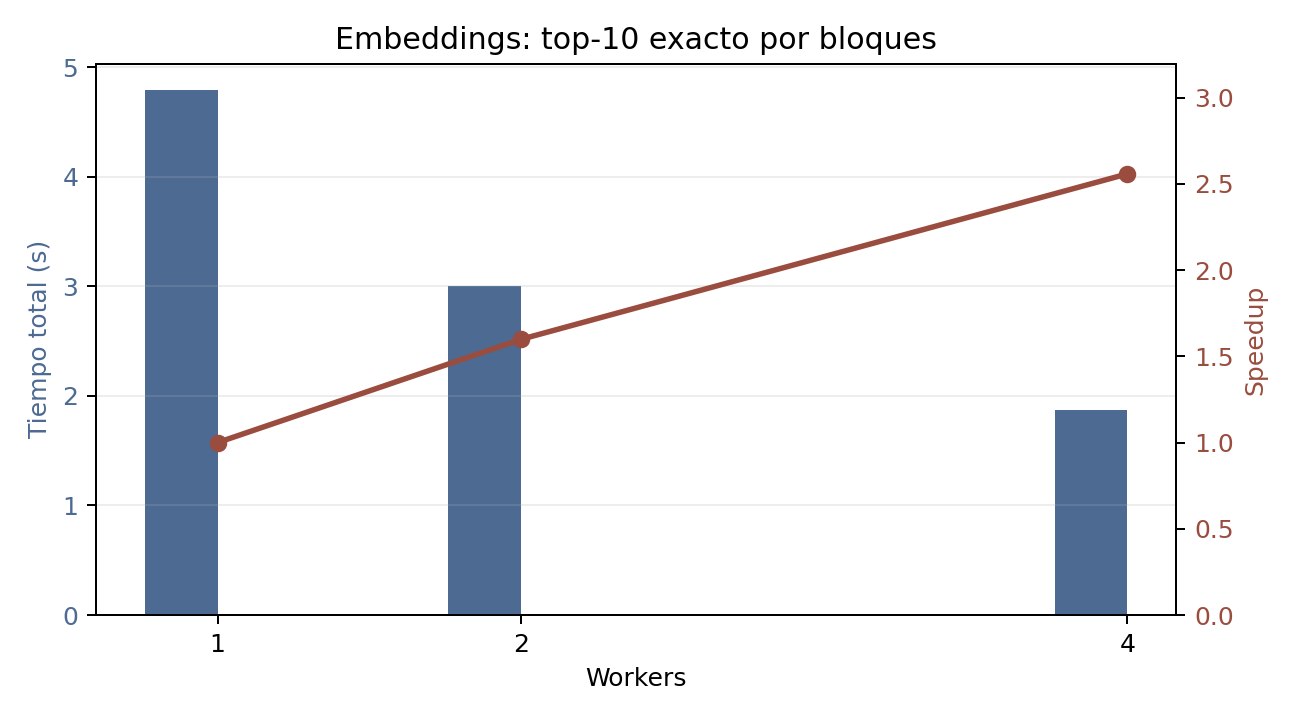
\includegraphics[width=0.82\linewidth]{figuras/embeddings_tiempo_speedup.png}
    \caption{Tiempo y speedup del top-10 exacto por bloques para embeddings.}
\end{figure}

El speedup mejora al pasar a 2 y 4 workers, pero no llega a ser lineal. Hay costo de crear procesos, coordinar tareas y devolver matrices top-\(k\). Además, las multiplicaciones por bloque ya usan memoria y caché de forma intensa, por lo que el ancho de banda disponible también limita.

\subsection{Riesgos y alternativas}

Si el número de vectores sube a millones, el enfoque exacto deja de ser práctico aunque se use por bloques. Ahí habría que evaluar aproximaciones como índices ANN, HNSW o IVF, midiendo recall@10 contra una muestra exacta. Si se trabaja en GPU, la estrategia de bloques seguiría siendo útil, pero habría que cuidar transferencias CPU-GPU y memoria de dispositivo. Si los vectores no estuvieran normalizados, habría que normalizar antes o guardar normas para no confundir producto punto con coseno.

\section{Discusión transversal}

La revisión de la parte individual ayudó a evitar una solución grupal escrita solo desde el resultado final. En vez de elegir una biblioteca y justificarla después, partimos de las dudas que aparecieron en la prueba: dónde hay dependencia de datos, qué se puede repartir sin sincronización fina y qué métrica permite defender que la versión paralela realmente aporta.

Los tres ejercicios muestran que el paralelismo no se decide por moda de herramienta. En OpenMP el problema es memoria compartida y reducción controlada; en logs el punto crítico es separar I/O-bound de CPU-bound y medir el efecto del GIL; en embeddings el problema real no es solo paralelizar un doble ciclo, sino controlar memoria y mantener top-\(k\) sin guardar todo.

También aparece el mismo patrón de fondo: más workers no garantizan mejor eficiencia. En OpenMP la eficiencia bajó con 8 hilos por presión de memoria y combinación. En logs, 8 procesos mejoraron tiempo, pero pagaron serialización y coordinación. En embeddings, 4 workers aceleraron, aunque el retorno marginal cayó. Esa lectura es más útil que reportar solamente el menor tiempo.

\section{Conclusiones}

La estrategia grupal más defendible para normalización fue OpenMP con arreglos privados por hilo y combinación final, porque evita condiciones de carrera sin introducir una región crítica dentro del bucle masivo. Para logs, la mejor decisión no fue usar hilos por defecto, sino comparar etapas: en nuestra medición el parseo y la agregación hicieron que procesos e híbrido fueran superiores. Para embeddings, el diseño por bloques permitió resolver el tamaño completo pedido con memoria temporal pequeña y top-10 exacto.

Las mediciones no buscan prometer aceleración universal. En otro disco, otra versión de Python, otro compilador o datos con distinta cardinalidad, los puntos óptimos pueden cambiar. Lo importante es que las decisiones quedan justificadas por diagnóstico, particionamiento, sincronización, benchmark y límites claros.

\section*{Registro de entorno y ejecución}
\addcontentsline{toc}{section}{Registro de entorno y ejecución}

\begin{itemize}[itemsep=0.1cm]
    \item Sistema operativo: Microsoft Windows 11 Home Single Language 10.0.26200.
    \item CPU: AMD Ryzen 7 6800H with Radeon Graphics.
    \item Núcleos físicos: 8; hilos lógicos: 16.
    \item RAM aproximada: 15,26 GiB.
    \item Python: 3.13.5.
    \item Compilador C/C++: MinGW-W64 GCC/G++ 13.2.0.
    \item Material OpenMP de referencia: paquete portable \texttt{OpenMP.rar} entregado por el profesor, con instructivo \texttt{Leeme.txt}, configuración VSCode y ejemplos base de suma y conteo de primos.
    \item OpenMP: compilación con \texttt{-fopenmp}; mediciones con \texttt{OMP\_NUM\_THREADS=1,2,4,8}.
    \item Repeticiones: OpenMP 3 repeticiones por configuración en tabla comparativa; logs 2 repeticiones con una corrida de calentamiento; embeddings 1 repetición en el tamaño completo y 2 repeticiones en escala intermedia.
    \item Anexos OpenMP: \texttt{openmp\_normalizacion\_50m.csv} y \texttt{openmp\_normalizacion\_50m\_raw.csv}.
    \item Otros anexos: \texttt{pipeline\_logs\_16mib.csv} y \texttt{embeddings\_topk\_20000.csv}.
\end{itemize}

\section*{Declaración de apoyo y uso de herramientas}
\addcontentsline{toc}{section}{Declaración de apoyo y uso de herramientas}

Se usaron fuentes públicas y documentación técnica para contrastar decisiones de implementación. También se utilizó asistencia computacional para apoyar búsqueda de referencias, organización del informe, revisión de código y preparación de scripts de benchmark. El grupo revisó, adaptó y ejecutó los programas localmente, dejando los comandos y resultados en anexos.

\begin{thebibliography}{9}

\bibitem{opensky}
The OpenSky Network. Scientific Datasets. Disponible en:
\url{https://opensky-network.org/data/scientific}

\bibitem{rba}
DAS Group. RBA Dataset. Disponible en:
\url{https://github.com/das-group/rba-dataset}

\bibitem{azurelogs}
Microsoft Learn. Application Gateway Access Logs schema. Disponible en:
\url{https://learn.microsoft.com/en-au/azure/azure-monitor/reference/tables/agwaccesslogs}

\bibitem{sift}
Hugging Face. SIFT1M dataset card. Disponible en:
\url{https://huggingface.co/datasets/maknee/sift1m}

\bibitem{openmp}
OpenMP Architecture Review Board. OpenMP API Specification. Disponible en:
\url{https://www.openmp.org/specifications/}

\bibitem{pythonthreading}
Python Software Foundation. \textit{threading} documentation. Disponible en:
\url{https://docs.python.org/3/library/threading.html}

\bibitem{pythonfutures}
Python Software Foundation. \textit{concurrent.futures} documentation. Disponible en:
\url{https://docs.python.org/3/library/concurrent.futures.html}

\bibitem{pythonmp}
Python Software Foundation. \textit{multiprocessing} documentation. Disponible en:
\url{https://docs.python.org/3/library/multiprocessing.html}

\bibitem{pacheco}
Pacheco, P. (2011). \textit{An Introduction to Parallel Programming}. Morgan Kaufmann.

\end{thebibliography}

\end{document}
